
This chapter is based on Refs. \cite{eli-daw-book}
and \cite{lich-book}.

\beq
[\vec{H},\;\cdot\;]E_{\vec{\alp}}
=
[\vec{H}, E_{\vec{\alp}}]= \vec{\alp} E_{\vec{\alp}}
\eeq

\beq
\vec{H}\ket{j, \vec{m}}= \vec{m}\ket{j, \vec{m}}
\eeq

Vectors like $\vec{\alp}$ and $\vec{m}$ live in root space $\RR^r$,
where $r$ is the rank of the Lie algebra.

brakets like $\ket{j, \vec{m}}$ live in multiplet space 
$\RR^d$, where $d$ is the dimesion of the irrep

\begin{figure}[h!]
\centering
\includegraphics[width=2.5in]
{weight-diagrams/weight-roots-relation.png}
\caption{Relationship between 2 weights $\vec{m}$ and $\vec{m}'$.}
\label{fig-weight-roots-relation}
\end{figure}



\begin{claim}
For any weight $\vec{m}$ and
root $\vec{\alp}$,
if $k$ is an integer and

\beq k = -\;\frac{2\vec{m}\cdot \vec{\alp}}{\vec{\alp}\cdot\vec{\alp}}
\eeq
then

\beq
\vec{m}'=\vec{m} + k\vec{\alp}
\eeq
is a weight
with the same eigenvalue multiplicity as $\vec{m}$.
\end{claim}
\proof
\qed


\section{WD for $SU(2)$}

\beq
m=-j, -j+1, \ldots, j-1, j
\eeq

\section{WD for $SU(3)$}

\beq
\ket{1}=\begin{pmatrix}
1
\\
0
\\
0
\end{pmatrix}
,\quad
\ket{2}=\begin{pmatrix}
0
\\
1
\\
0
\end{pmatrix}
,\quad
\ket{3}=\begin{pmatrix}
0
\\
0
\\
1
\end{pmatrix}
\eeq

\beq
\sqrt{3}E_1=T_+=\ket{1}\bra{2},\quad
\sqrt{3}E_{-1}=T_- =\ket{2}\bra{1}
\eeq

\beq
\sqrt{3}E_3=U_+ = \ket{2}\bra{3},\quad
\sqrt{3}E_{-3} = U_- = \ket{3}\bra{2}
\eeq

\beq
\sqrt{3}E_{-2}=V_+ = \ket{3}\bra{1},\quad
\sqrt{3}E_2=V_- = \ket{1}\bra{3}
\eeq

\beq
\sqrt{\frac{3}{2}}H_1=T_z = \frac{1}{2}
\left(
\ket{1}\bra{1}
-\ket{2}\bra{2}\right),
\quad
\sqrt{2}H_2=Y=
\frac{1}{3}
\left(
\ket{1}\bra{1}
+\ket{2}\bra{2}
-2\ket{3}\bra{3}
\right)
\eeq

\renewcommand{\arraystretch}{1.5}
\beq
\begin{pmatrix}
\sqrt{\frac{3}{2}}H_1
\\
\sqrt{2}H_2
\end{pmatrix}
\ket{1}
=
\begin{pmatrix}
T_z
\\
Y
\end{pmatrix}
\ket{1}
=
\begin{pmatrix}
\frac{1}{2}
\\
\frac{1}{3}
\end{pmatrix}
\ket{1}
=
\vec{m}(1)\ket{1}
\eeq

\beq
\begin{pmatrix}
\sqrt{\frac{3}{2}}H_1
\\
\sqrt{2}H_2
\end{pmatrix}
\ket{2}
=
\begin{pmatrix}
T_z
\\
Y
\end{pmatrix}
\ket{2}
=
\begin{pmatrix}
-\frac{1}{2}
\\
\frac{1}{3}
\end{pmatrix}
\ket{2}
=
\vec{m}(2)\ket{2}
\eeq

\beq
\begin{pmatrix}
\sqrt{\frac{3}{2}}H_1
\\
\sqrt{2}H_2
\end{pmatrix}
\ket{3}
=
\begin{pmatrix}
T_z
\\
Y
\end{pmatrix}
\ket{3}
=
\begin{pmatrix}
0
\\
-\frac{2}{3}
\end{pmatrix}
\ket{3}
=
\vec{m}(3)\ket{3}
\eeq
\renewcommand{\arraystretch}{1}

\begin{figure}[h!]
\centering
\includegraphics[width=4in]
{weight-diagrams/tuv-plus.png}
\caption{Roots of $SU(3)$.}
\label{fig-tuv-plus}
\end{figure}

\begin{figure}[h!]
\centering
\includegraphics[width=4in]
{weight-diagrams/weights-fundamental.png}
\caption{For $SU(3)$, roots in green and weights of fundamental rep in red.}
\label{fig-weights-fundamental}
\end{figure}

\begin{figure}[h!]
\centering
\includegraphics[width=2.4in]
{weight-diagrams/123-vecs.png}
\caption{$\ket{1}, \ket{2}, \ket{3}$ 
vectors, and operators that act on them. $E_{-i}$ in opposite direction 
as $E_i$ for $i=1,2,3$.}
\label{fig-123-vecs}
\end{figure}